\parindent=0em
\subsection{Hololens 2}
\label{HoloLens2Dispositivo}
\noindent

Las \textit{Microsoft HoloLens 2} son un casco desarrollado por Microsoft que salió al mercado por primera vez el día 7 de Noviembre de 2019, es el dispositivo sucesor a las Microsoft Hololens de 2016.


\begin{figure}[htbp]
\centering
    \hspace{-4mm}
    \begin{minipage}{0.5\textwidth}
        \centering
        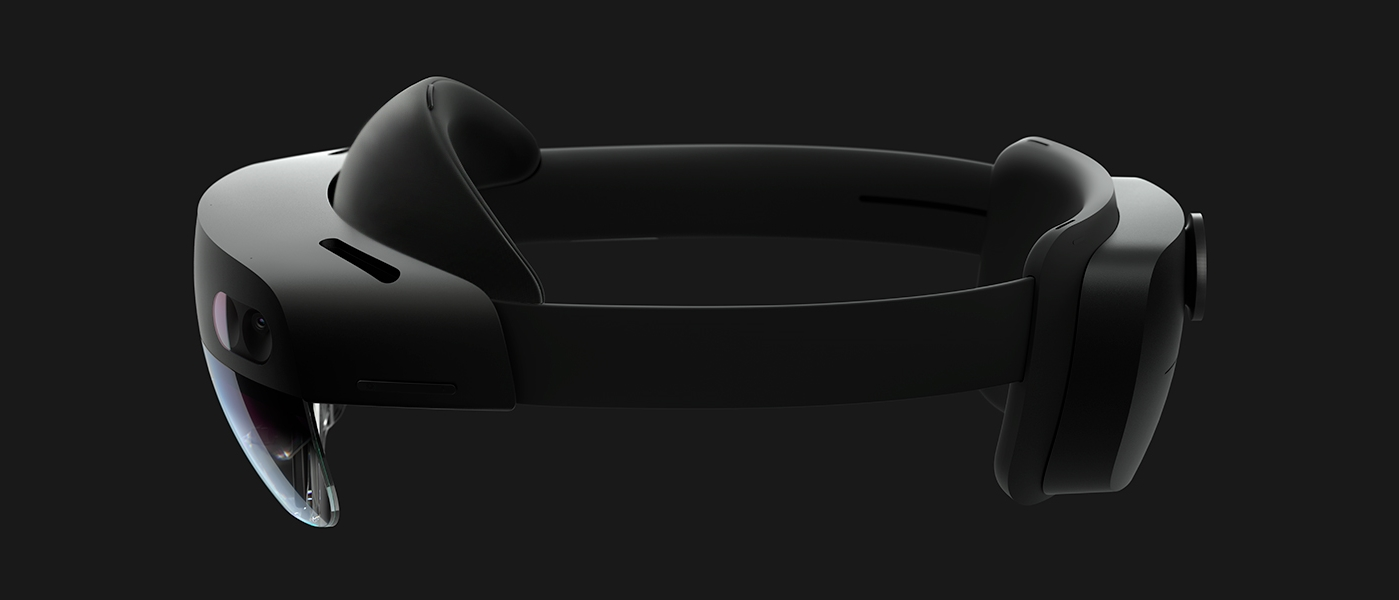
\includegraphics[scale=0.2]{Images/Estado del arte/hololens2_2.jpeg}\\
        (a) Vista lateral.
    \end{minipage}
    \begin{minipage}{0.5\textwidth}
        \centering
        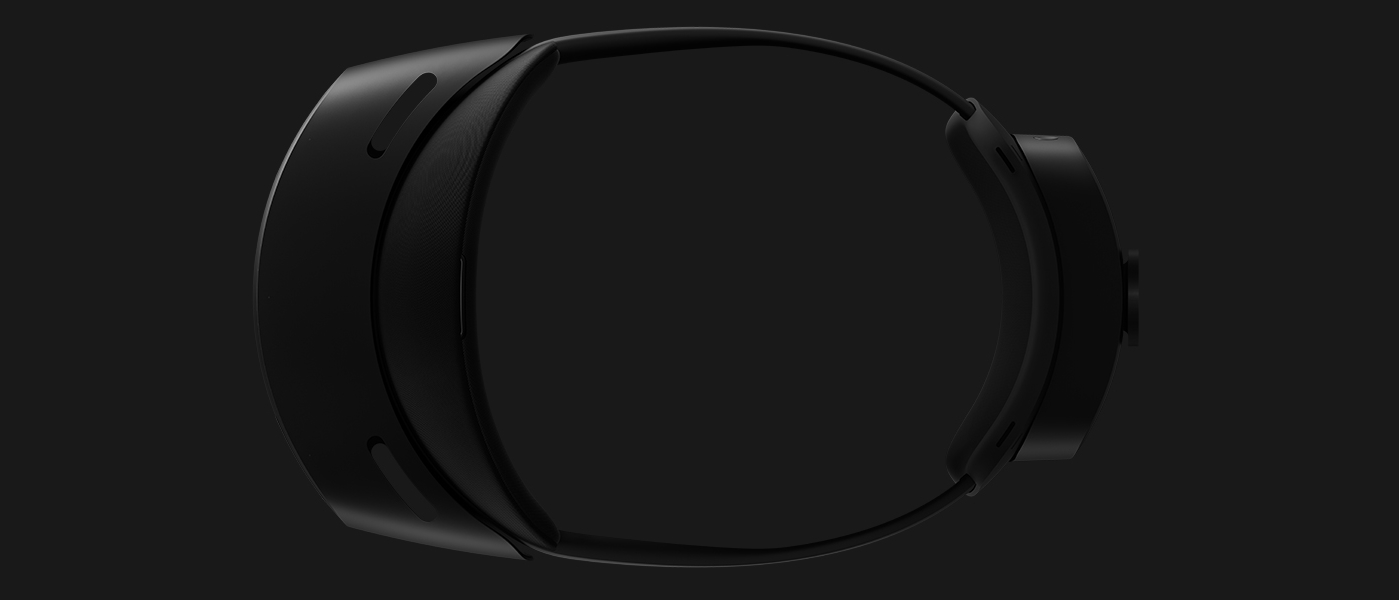
\includegraphics[scale=0.2]{Images/Estado del arte/hololens2_3.jpeg}\\
       (b) Vista superior.
    \end{minipage}\\
    \caption{Vistas de las Microsoft HoloLens 2\textsuperscript{\ref{hololens2footer}}.}
    \label{fig:vistasHoloLens2}
\end{figure}


Microsoft Hololens 2 utiliza los servicios de cloud y la IA de Microsoft, además, está diseñado con un sistema ergonómico de tal forma que no hay necesidad de quitarse las gafas ya que se coloca directamente sobre ellas (figura~\ref{fig:hololensErgonomicas}).\\
\begin{wrapfigure}{r}{.5\textwidth}
  \centering
    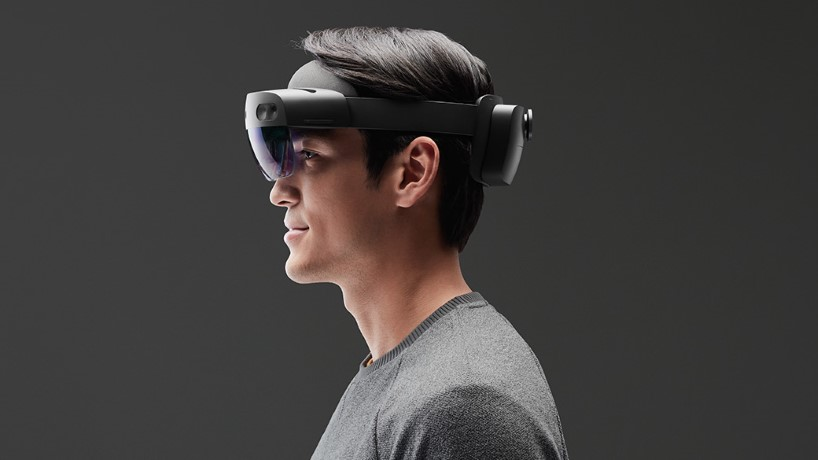
\includegraphics[scale=0.28]{Images/Estado del arte/hololens2_1.jpeg}
  \caption{Diseño ergonómico del dispositivo\textsuperscript{\ref{hololens2footer}}
  }
  
  \label{fig:hololensErgonomicas}
\end{wrapfigure}

Respecto a las especificaciones técnicas del casco se pueden destacar las siguientes relacionadas con los sensores: cuatro cámaras de luz visible para el seguimiento de la cabeza, dos cámaras de infrarrojos para el movimiento de los ojos y un sensor de profundidad de 1 mega píxel, además de contar con acelerómetro, giroscopio y magnetómetro.\\



El dispositivo cuenta también con seguimiento de mano, seguimiento de ojos y controles por voz.
Por último, las Microsoft HoloLens 2 tienen un peso de 566 gramos y utilizan un sistema operativo holográfico de Windows.

Actualmente están disponibles para empresas y desarrolladores, su precio depende de la elección entre distintos paquetes:

\begin{itemize}
    \item \textbf{Solo el dispositivo:} 3,500 dólares.
    \item \textbf{Dispositivo con asistencia remota:} El coste del dispositivo y 500 dólares al mes, incluye asistencia remota los 365 días.
    \item \textbf{Paquete de desarrollador:} Coste del dispositivo añadido a 99 dólares por mes, este paquete incluye Unity Pro y un crédito de 500 dólares para Azure.
\end{itemize}

\footnotetext[1]{\label{hololens2footer}{Imágenes y especificaciones obtenidas de \url{https://www.microsoft.com/es-es/hololens/hardware}.}}



